  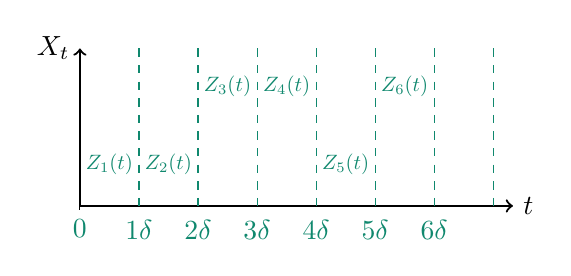
\begin{tikzpicture}[scale=0.5]
 
     % Axis
     \draw[<->, thick] (0,4) node (yaxis) [left] {$X_t$} 
        |- (11,0) node (xaxis) [right] {$t$} ;
     % Dashed grid
     \foreach \t in {1, 2, 3, 4, 5, 6} 
        \draw[dashed, color=PineGreen] (1.5*\t cm, 4) -- (1.5*\t cm, -3pt) 
                         node[anchor=north] {$\t \delta$};

     \draw[color=PineGreen] plot[smooth] file {tikz/data.dat};

     \draw (0,0) -- (0,-3pt) node[below, color= PineGreen] {0};
     \draw[dashed, color=PineGreen] (1.5*7,4) -- (1.5*7,-3pt) 
                         node[below] {};%$T+\delta$

     \foreach \t in {1, 2, 5} 
        \draw[color=PineGreen] (-0.75+1.5*\t, 1.5) node[below, scale=0.75] {$Z_\t(t)$};
        
     \foreach \t in {3, 4, 6} 
        \draw[color=PineGreen] (-0.75+1.5*\t, 3.5) node[below, scale=0.75] {$Z_\t(t)$};
     
  \end{tikzpicture} 
